%!TEX root = ../Allnew-Workspace.tex
\mychapter{미분법}{}
\section{평균변화율과 순간변화율}
함수 $y=f\left( x \right) $에서 $x$의 값이 $a$에서 $b$까지 변할 때, $y$의 값은 $f\left( a \right) $에서 $f\left( b \right) $까지 변합니다. 이때 $x$의 값의 변화량 $b-a$를 $x$의 \term{증분}{}, 이에 대한 $y$의 값의 변화량 $f\left( b \right) - f\left( a \right) $를 $y$의 \term{증분}{}이라 하고, 이것을 기호로 각각 $\Delta x$, $\Delta y$와 같이 표기합니다. 이를 등식으로 나타내면 다음과 같습니다.
\begin{align*}
    \Delta &x = b-a \\
    \Delta &y = f\left( b \right) -f\left( a \right)
\end{align*}
일반적으로 $\Delta x$에 대한 $\Delta y$의 비율을 `$x$의 값이 $a$에서 $b$까지 변할 때의 함수 $y=f\left( x \right) $의 \term{평균변화율}{}'이라고 합니다. 이는 곡선 $y=f\left( x \right) $ 위의 두 점 $\xy[A]{a}{f(a)}$, $\xy[B]{b}{f\left( b \right) }$를 지나는 직선의 기울기와 같으며, 등식으로 나타내면 다음과 같습니다.
\begin{align*} \dfrac{\Delta y}{\Delta x} = \dfrac{f\left( b \right) - f\left( a \right) }{b-a} = \dfrac{f\left( a+\Delta x \right) - f\left( a \right) }{\Delta x}\end{align*}
이때 $\Delta x$라는 기호는 경제적이지 않으므로, 주로 문자 $h$로 대체되어 다음과 같이 표현합니다. 
\begin{align*} \dfrac{\Delta y}{\Delta x} =  \dfrac{f\left( a+h \right) - f\left( a \right)  }{h}\end{align*}

\section{미분계수}
`$x$의 값이 $a$에서 $a+ \Delta x$까지 변할 때의 함수 $y=f\left( x \right) $의 평균변화율'인 $\dfrac{\Delta y}{\Delta x}$에 대하여, $\Delta x \to 0$일 때 `평균변화율의 극한값'인
\begin{align*} \lim_{\Delta x \to 0} \dfrac{\Delta y}{\Delta x} \end{align*}
가 존재하는 경우가 있습니다. 이러한 경우 함수 $y=f\left( x \right) $가 $x=a$에서 \term{미분가능}{}하다고 합니다. 이때 이 극한값을 함수 $y=f\left( x \right) $의 $x=a$에서의 \term{순간변화율}{} 또는 $x=a$에서의 \term{미분계수}{}라 하고, 기호로 $f'\left( a \right) $와 같이 나타냅니다. 이를 등식으로 나타내면 다음과 같습니다.
\begin{align*} \lim_{\Delta x \to 0} \dfrac{\Delta y}{\Delta x} = \lim_{\Delta x \to 0} \dfrac{f\left( a+ \Delta x \right) - f\left( a \right)  }{\Delta x}  = \lim_{h \to 0} \dfrac{f\left( a+h \right) - f\left( a \right)  }{h} =f'(a)\end{align*}

$f'\left( a \right) $를 표현하는 다른 방법도 있습니다. 두 점 $\xy[A]{a}{f\left( a \right)}$, $\xy[P]{x}{f\left( x \right) }$을 이용하여 다음과 같이 표현하는 것입니다.
\begin{align*} \lim_{x \to a} \dfrac{f\left( x \right) - f\left( a \right)  }{x - a} = f'\left( a \right) \end{align*}
\clearpage
\section{평균변화율과 순간변화율의 기하학적 의미}
\begin{center} 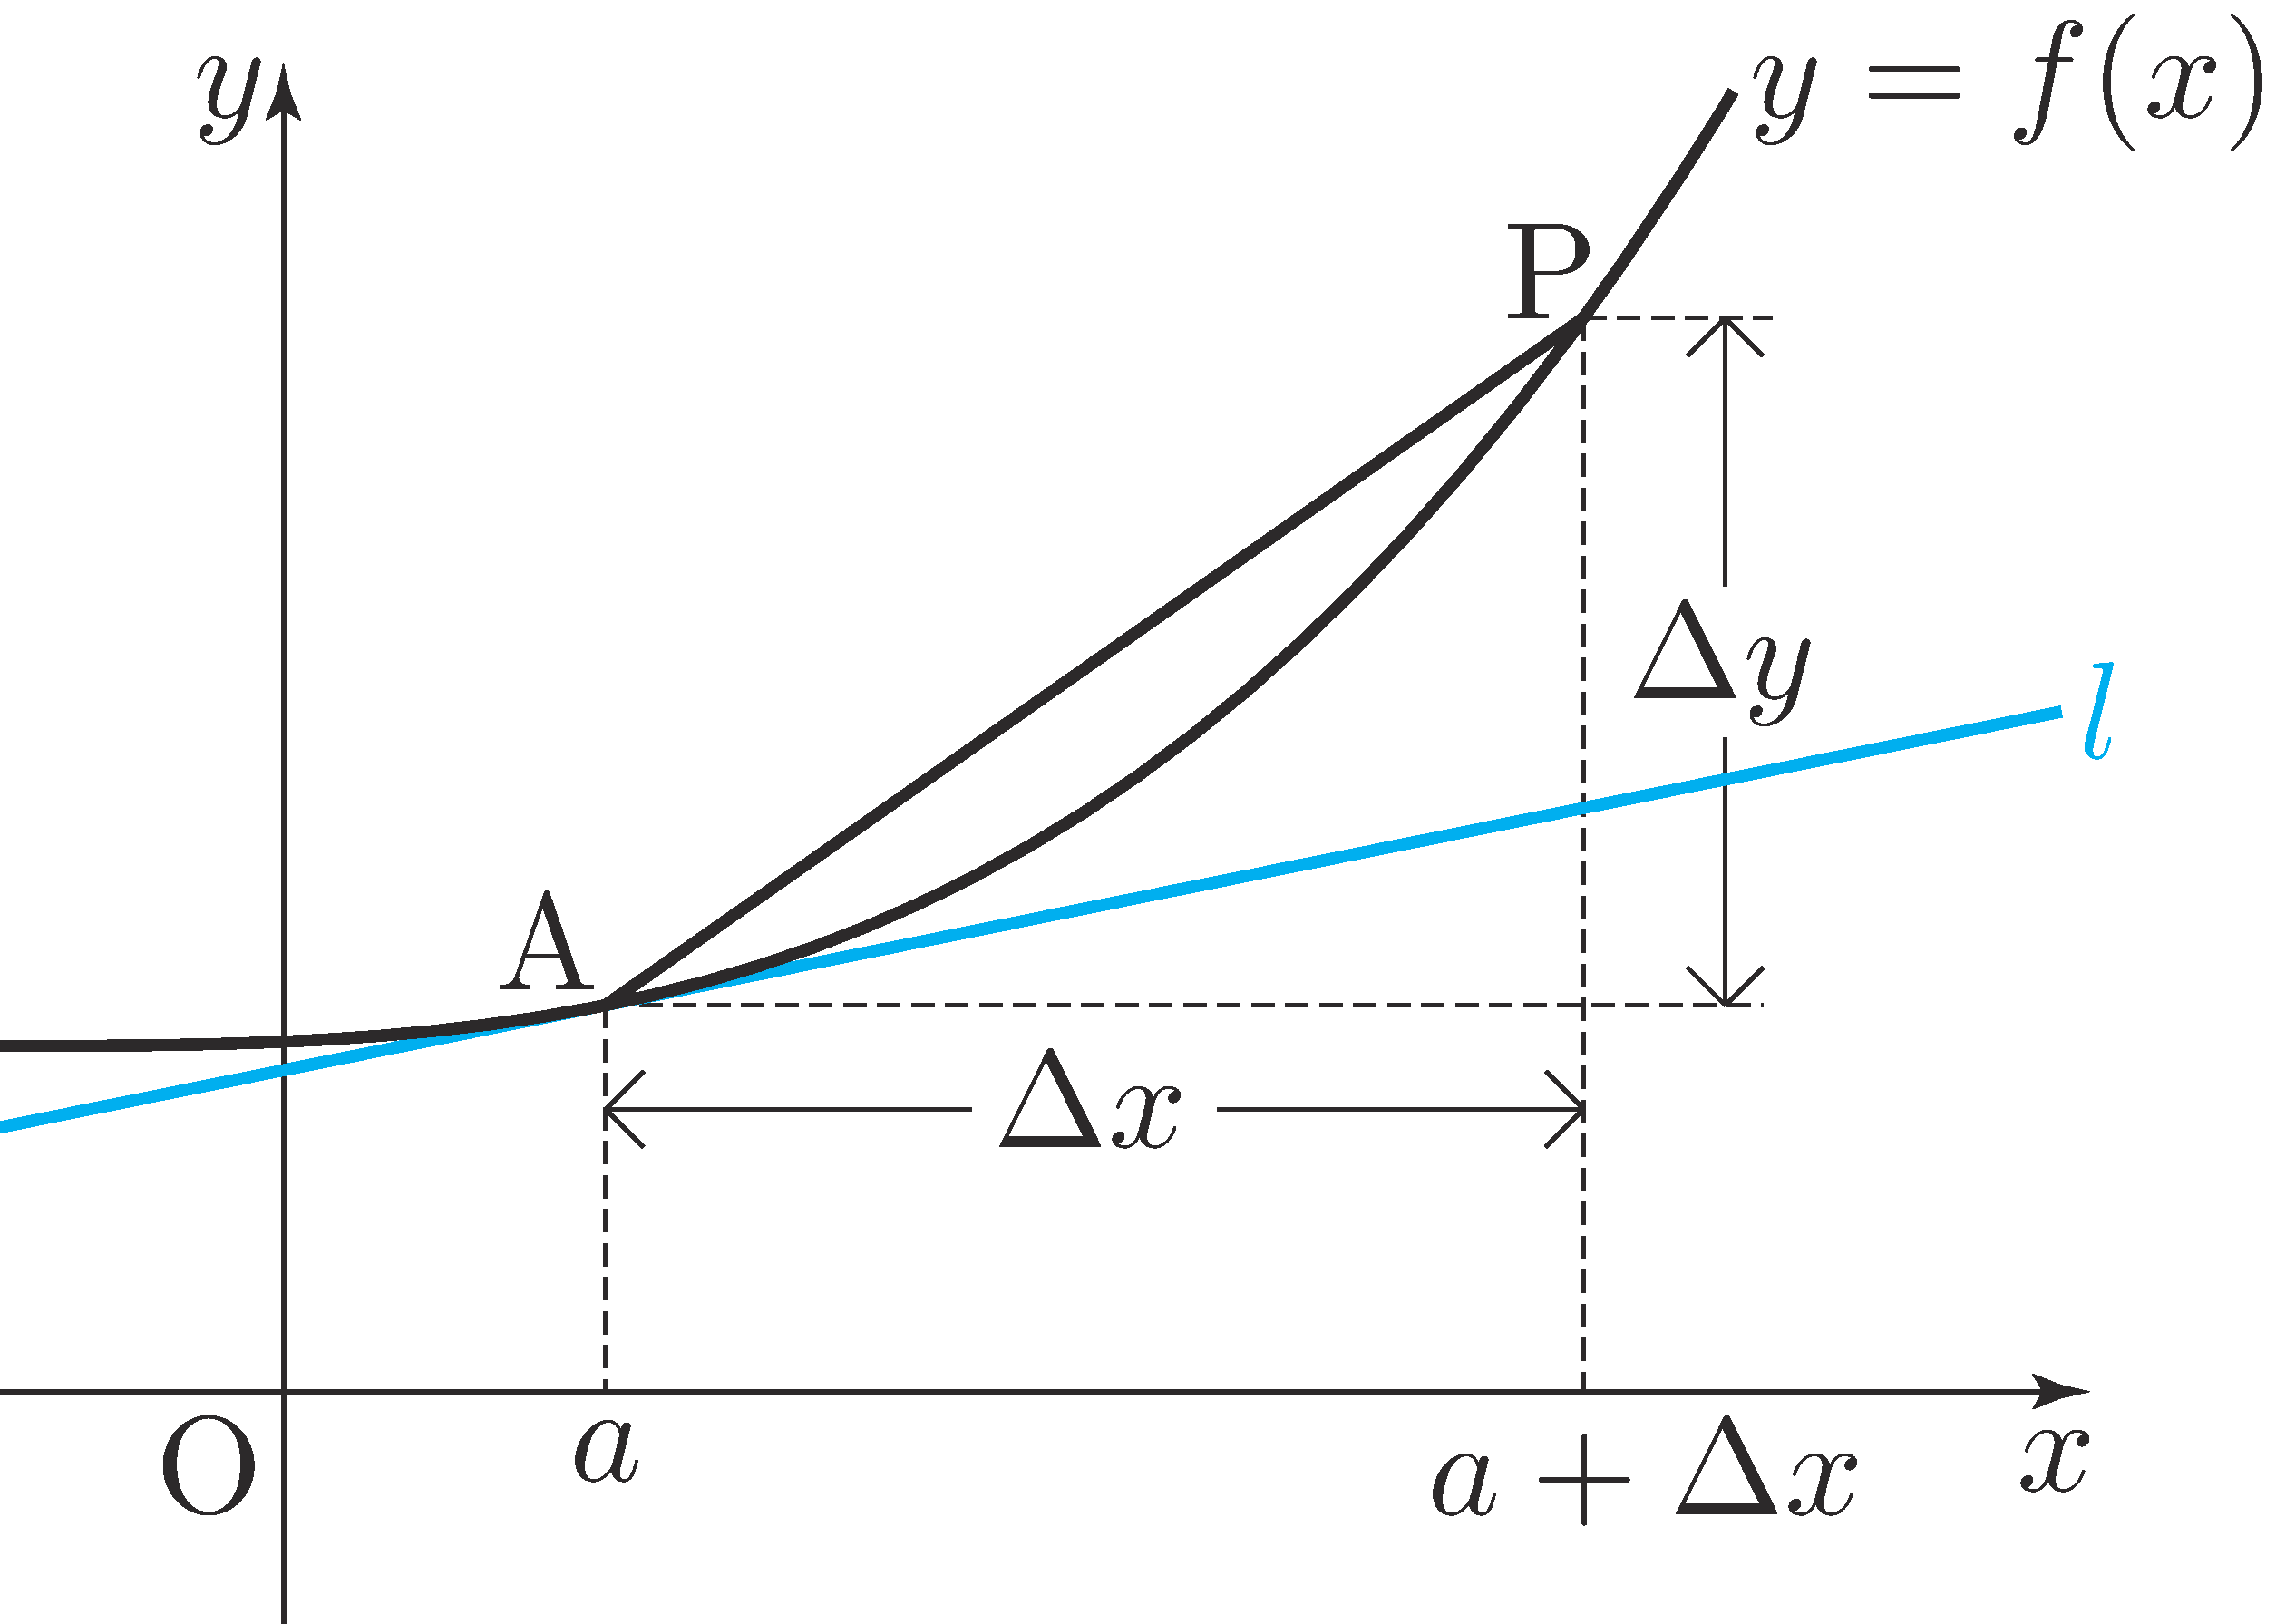
\includegraphics[scale=\pgfkeysvalueof{picsize}]{DBs/pic/zerr_01.pdf}\\
	\end{center}순간변화율은 평균변화율의 극한값이므로, 둘의 기하학적 의미를 살펴보겠습니다. `$x$의 값이 $a$에서 $a+ \Delta x$까지 변할 때의 함수 $y=f\left( x \right) $의 평균변화율'인 $\dfrac{\Delta y}{\Delta x}$는 \mbox{두 점 $\xy[A]{a}{f\left( a \right) }$,} $\xy[P]{a+\Delta x}{f\left( a+\Delta x \right) }$를 지나는 직선 $\mrm{AP}$의 기울기를 의미합니다. 

이때 점 $\mrm{A}$를 고정하고\mn{즉 $a$를 상수로 취급하고}{} $\Delta x \to 0$인 상황을 관찰하면, 점 $\mrm{P}$는 곡선 $y=f\left( x \right) $를 따라 점 $\mrm{A}$에 한없이 가까워지고, 직선 $\mrm{AP}$는 점 $\mrm{A}$를 지나는 어떤 직선 $l$에 한없이 가까워짐을 \dotemph{직관적으로} 알 수 있습니다. 이 직선 $l$을 곡선 $y=f\left( x \right) $ 위의 점 $\mrm{A}$에서의 \term{접선}{}이라고 하고, 점 $\mrm{A}$를 \term{접점}{}이라고 합니다.\mn{어떤 팽팽한 실 위에 정지한 채 놓여 있는 탁구공과 실의 관계를 생각하면, 탁구공과 실이 맞닿아 있는 유일한 그 점이 접점, 실이 접선이라 생각할 수 있습니다.}{}

지금까지 살펴본 바에 따르면, 함수 $y=f\left( x \right) $의 $x=a$에서의 미분계수 $f'\left( a \right) $는 곡선 $y=f\left( x \right) $위의 점 $\xy[A]{a}{f\left( a \right) }$에서의 접선의 기울기와 같음을 \dotemph{직관적으로} 알 수 있습니다.

\section{미분가능과 연속의 관계}

\subsection{미분가능하면 연속인가?}
함수 $f\left( x \right) $가 $x=a$에서 미분가능하면 $x=a$에서 미분계수가 존재하므로 다음이 성립합니다.
$f'\left( a \right) = \lim_{x \to a} \dfrac{f\left( x \right) -f\left( a \right) }{x-a} \cdots \text{①}$
이때 $\lim_{x \to a} \left( x-a \right) = 0 \cdots \text{②}$이므로 ①과 ②를 서로 곱하면, 함수의 극한의 성질에 의해 다음이 성립합니다.
\begin{align*}
    \lim_{x \to a} \dfrac{f\left( x \right) -f\left( a \right) }{x-a} \times \lim_{x \to a} \left( x-a \right)
    &= f'\left( a \right) \times 0\\
    \lim_{x \to a} \left\{ \dfrac{f\left( x \right) -f\left( a \right) }{x-a}\times \left( x-a \right) \right\} &= 0 \\
    \lim_{x \to a} \left\{ f\left( x \right) -f\left( a \right) \right\}   &= 0 \\
    \lim_{x \to a} f\left( x \right) - f\left( a \right)    &= 0 \\
    \lim_{x \to a} f\left( x \right) &= f\left( a \right) 
\end{align*}
이는 함수 $f\left( x \right) $가 $x=a$에서 연속임을 의미합니다. 따라서 `함수 $f\left( x \right) $가 $x=a$에서 미분가능하면 $x=a$에서 연속'입니다.
\clearpage
\subsection{연속이면 미분가능한가? \& 첨점의 정의}
앞서 배운 명제의 역인\begin{center}
    함수 $f\left( x \right) $가 $x=a$에서 연속이면 $x=a$에서 미분가능하다
\end{center}는 거짓입니다. 예를 들어 함수 $f\left( x \right) =\abs{x}$는 $x=0$에서 연속이지만 $\lim_{h \to 0} \dfrac{\abs{0+h} - \abs0}{h}=\lim_{h \to 0} \dfrac{\abs{h}}{h}$의 값이 존재하지 않으므로 $x=0$에서 미분가능하지 않습니다. 이처럼 함수 $y=f\left( x \right) $가 $x=a$에서 연속이지만 미분가능하지 않을 때, 점 $\xy[A]{a}{f\left( a \right) }$를 첨점이라 부르기로 합시다.


\section{도함수}
\subsection{미분가능한 함수의 정의}
함수 $y=f\left( x \right) $가 정의역에 속하는 모든 $x$의 값에서 미분가능할 때, 함수 $f\left( x \right) $를 \term{미분가능한 함수}{}라고 합니다.

미분가능한 함수의 정의역은 반드시 열린구간입니다. 닫힌구간 $\CCI ab$에서 정의된 경우 $x=a$, $x=b$에서 미분가능하지 않고, 반닫힌구간 $\COI ab$나 $\OCI ab$에서 정의된 경우 각각 $x=a$, $x=b$에서 미분가능하지 않기 때문입니다.

\subsection{도함수와 원함수의 정의}
임의의 실수 $a$에 대하여 함수 $f\left( x \right) = x^2$의 $x=a$에서의 미분계수 $f'\left( a \right) $는 $f'\left( a \right) = 2a $입니다. 따라서 실수 $a$의 값에 따라 미분계수 $f'\left( a \right) $의 값이 \dotemph{오직 하나씩} 정해집니다. 따라서 함수 $f\left( x \right) $의 정의역에 포함된 원소 $k$와, 그 함수 $f\left( x \right) $의 $x=k$에서의 미분계수 $f'\left( k \right) $를 대응시키는 새로운 함수 $f'\left( x \right) $를 생각할 수 있습니다.\mn[-6em]{이때 $f\left( x \right) $의 정의역이 열린구간 $\OOI ab$이면 $f'\left( x \right) $의 정의역도 열린구간 $\OOI ab$입니다. $f\left( x \right) $의 정의역이 닫힌구간 $\CCI{a}{b}$이나 반열린구간이면 구간의 끝은 제외하고 나머지 열린구간 $\OOI ab$를 정의역으로 합니다.}{} 이때 함수 $f'\left( x \right) $의 함수식은 다음과 같습니다.
\begin{align*} \lim_{h \to 0}\dfrac{f\left( x+h \right)  - f\left( x \right) }{ h}\end{align*}
이러한 함수 $f'\left( x \right) $를 `함수 $f\left( x \right) $의 \term{도함수}{}'라 하고, 이것을 다음과 같이 표기합니다.\mn[1em]{단, $y'$과 $\dfrac{dy}{dx}$는 $y=f\left( x \right) $라 할 때 쓸 수 있는 표현입니다.}{}
\begin{align*}f'\left( x \right),\quad y',\quad \dfrac{dy}{dx} ,\quad \dfrac{d}{dx}f\left( x \right)\end{align*}
도함수 $f'\left( x \right) $는 태생부터 함수 $f\left( x \right) $와 매우 밀접한 관계를 가지므로, $f'\left( x \right) $를 중심으로 생각할 때 $f(x)$를 부를 적당한 명칭이 필요할 것입니다. 따라서 어떤 함수 $f(x)$의 도함수 $f'(x)$가 존재할 때, $f\left( x \right) $를 `$f'\left( x \right) $의 \iterm{원함수}{}'라 부르기로 합시다.
\clearpage
\subsection{도함수와 미분계수의 관계}
함수 $f\left( x \right) $의 $x=a$에서의 미분계수 $f'\left( a \right) $는 도함수 $f'\left( x \right) $의 식에 $x=a$를 대입한 것과 같습니다. 즉 미분계수를 구하는 방법은 직접 미분계수의 정의에 따라 구하는 방법과, 도함수를 구한 후 $x=a$를 대입하는 방법으로 나뉩니다.

도함수 $f'\left( x \right) $의 정의역은 반드시 원함수 $f\left( x \right) $의 정의역과 동일해야 함을 주의합시다. 예를 들어 정의역이 실수 전체의 집합인 함수 $f\left( x \right) = \abs{x}$와 $x \ne 0 $인 모든 실수 $x$에 대하여
\begin{align*} f'\left( x \right) = 
\begin{cases}
1 & \left( x > 0 \right) \\
-1 & \left( x < 0 \right) 
\end{cases}
\end{align*}
이 성립하기는 하지만, 이때 $f'\left( x \right) $를 도함수라고 부를 수는 없습니다. 원함수의 정의역에 속하는 원소인 $0$에 대하여 $f'\left( 0 \right) $이 정의되지 않기 때문입니다. 따라서 이때 $f'\left( x \right) $는 도함수라 불릴 수 없으며, 미분계수라는 표현을 써야 합니다.

\section{미분법}
\subsection{미분과 미분법의 정의}
함수 $f\left( x \right) $의 도함수를 구하는 것을 `함수 $f\left( x \right) $를 $x$에 대하여 \term{미분}{}한다'고 하며, 그 과정에서 행하는 계산 방법을 \term{미분법}{}이라고 합니다.

\subsection{미분법의 표기 : 뉴턴식 vs. 라이프니츠식}

미분법의 표현 방식은 두 가지로 나뉩니다. 하나는 미분할 함수를 괄호로 묶은 후 우측 상단에 $'$을 표현하는 방법(\iterm{뉴턴식}{})이고, 다른 하나는 분수와 유사한 표현을 이용해 어떤 변수에 대하여 미분하는지를 표현내는 방법(\iterm{라이프니츠식}{})입니다. 이를테면 두 함수 $t=f\left( x \right)$, $s=g\left( x \right)$의 곱으로 나타내어진 함수 $y =h\left( x \right) = f\left( x \right)g\left( x \right) =ts $에 대하여, `함수 $h\left( x \right)$를 변수 $x$로 미분한다'는 표현을 각각의 방식으로 나타내면 다음과 같습니다.
\begin{alignat*}{3}
\left\{ h\left( x \right) \right\}'
&= \left\{ f\left( x \right) g\left( x \right)  \right\}' &&\quad\Rightarrow
\quad&&h'\left( x \right)
= f'\left( x \right)g\left( x \right) + f\left( x \right) g'\left( x \right) \\
\dfrac{d}{dx} h\left( x \right) 
&=\dfrac{d}{dx} \left\{ f\left( x \right)g\left( x \right)  \right\}  &&\quad\Rightarrow
\quad&&\dfrac{dy}{dx}
=\dfrac{dt}{dx}s + t\dfrac{ds}{dx}
\end{alignat*}
뉴턴식은 한 변수로 나타내어진 경우에서 식을 표현하기 편리하고, 라이프니츠식은 여러 개의 변수가 등장했을 때 혼동 없이 식을 표현하기 편리합니다. \cnm{미적분}을 선택하지 않는다면 뉴턴식만 익숙해져도 무방하지만, \cnm{미적분}을 선택한다면 두 표기법에 모두 익숙해지도록 노력합시다.\mn{특히 `음함수 미분법'과 `매개변수로 나타낸 함수(매나함)의 미분법', 그리고 이를 후속 단원에서 응용할 때에는 줄곧 라이프니츠식만 사용할 정도로 라이프니츠식의 중요성이 높아집니다.}{}
\clearpage
\subsection{미분법}
\subsubsection{$y=c$와 $y=x^n$의 도함수}
상수 $c$에 대하여, 도함수의 정의를 이용하여 함수 $f\left( x \right) = c$의 도함수 $f'\left( x \right) $를 구하면 $f'\left( x \right) = 0$을 얻습니다.  자연수 $n$에 대하여, 도함수의 정의를 이용하여 함수 $f\left( x \right) = x^n$의 도함수 $f'\left( x \right) $를 구하면 $f'\left( x \right) = nx^{n-1}$을 얻습니다. 
\subsubsection{함수의 실수배, 합, 차, 곱}
미분가능한 두 함수 $f\left( x \right) $, $g\left( x \right) $와 상수 $c$에 대하여, 도함수의 정의를 이용하여 함수 $cf\left( x \right) $, $f\left( x \right)+g\left( x \right)  $, $f\left( x \right) - g\left( x \right) $, $f\left( x \right)g\left( x \right)  $의 도함수를 구하면 각각 다음과 같습니다.
\begin{align*}
\left\{ cf\left( x \right)  \right\} '
&= cf'\left( x \right) \\
\left\{  f\left( x \right) \pm g\left( x \right) \right\}'
&= f'\left( x \right) \pm g'\left( x \right) \\
%\left\{  f\left( x \right) - g\left( x \right) \right\}'
%&= f'\left( x \right) - g'\left( x \right) \\
\left\{  f\left( x \right)g\left( x \right) \right\}'
&= f'\left( x \right)g\left( x \right)  + f\left( x \right) g'\left( x \right)
\end{align*}


\subsection{미분법의 활용}
\subsubsection{다항함수의 도함수}
다항함수 $f\left( x \right) = a_n x^n + a_{n-1}x^{n-1} + \cdots + a_2x^2 + a_1x + a_0 = \sum_{k=0}^n a_k x^k$는 미분가능한 함수인 상수함수 $y=a_n$과 함수 $y=x^n$의 실수배, 합, 차로 나타내어집니다. 따라서 미분법을 이용하여 $f'\left( x \right) $를 구하면 다음과 같습니다. (복부호 동순)
\begin{align*} f'\left( x \right) = na_nx^{n-1} + (n-1)a_{n-1}x^{n-2} + \cdots + 2a_2x + a_1= \sum_{k=1}^{n} ka_k x^{k-1} \end{align*}

\section{도함수의 활용}
\subsection{접선의 방정식}\term[함수]{접선의 방정식}{0}
$x=a$에서 미분가능한 함수 $f\left( x \right) $에 대하여 곡선 $y=f\left( x \right) $ 위의 점 $\xy{a}{f\left( a \right) }$에서의 접선의 방정식은 $y=f'\left( a \right) \left( x-a \right) +f\left( a \right) $입니다.
\subsection{함수의 증감성 분석, 그리고 방정식과 부등식의 풀이}
도함수는 함수의 증감성과 연관이 있습니다. 함수의 증감성이 무엇인지, 그리고 증감성과 도함수가 어떤 연관성을 가지고 있는지, 이를 방정식과 부등식을 푸는 데 어떻게 활용할 수 있는지에 대해서는 뒤에서 다룹니다.
\subsection{물리학(위치, 속도, 가속도)}
위치, 속도, 가속도 등의 물리학 개념을 미분으로 설명할 수 있습니다. \cnm{수학 II}에서는 수직선 위의 물리학만 다루며, 자세한 내용은 Calc에서 다룹니다.